\documentclass[conference]{IEEEtran}
\IEEEoverridecommandlockouts
% The preceding line is only needed to identify funding in the first footnote. If that is unneeded, please comment it out.
\usepackage{cite}
\usepackage{amsmath,amssymb,amsfonts}
\usepackage{algorithmic}
\usepackage{graphicx}
\usepackage{textcomp}
\usepackage{xcolor}
\def\BibTeX{{\rm B\kern-.05em{\sc i\kern-.025em b}\kern-.08em
		T\kern-.1667em\lower.7ex\hbox{E}\kern-.125emX}}
\begin{document}
	
	\title{\LARGE{Autonomous Garbage Collector Rover Using Image Processing}\\
		{\footnotesize \textsuperscript{}Autonomously and Manually Controlled Garbage Collector Rover Using Image Processing}
	}
	
	\author{
		\IEEEauthorblockN{1\textsuperscript{st} Sarhan Osman Bhuiya}
		\IEEEauthorblockA{\textit{ECE Department} \\
			\textit{North South University}\\
			Dhaka, Bangladesh \\
			sarhanbhuiya07@gmail.com}
	
		\and
		\IEEEauthorblockN{2\textsuperscript{nd} Given Name Surname}
		\IEEEauthorblockA{\textit{dept. name of organization (of Aff.)} \\
			\textit{name of organization (of Aff.)}\\
			City, Country \\
			email address}
		
	}
	
	\maketitle
	
	\begin{abstract}
		We are presenting a smart robot that could present a viable solution towards efficient waste management which is based on embedded, digital image processing. The system is designed so that it can automatically detect and collect the garbage. This report describes the basic idea of detection and collection. The detection is done by using the image processing model SSD Mobilenet v2. The real time video taken by the USB camera will be processed by the Raspberry Pi.  For each frame taken, Raspberry Pi will detect any garbage present in the frame and send signals to the robot. Our robot will calculate its position, calibrate the motors according to the position of the garbage so that it will go to the acquired position and collect the garbage. The collected garbage will be categorized as Paper, Plastic, Metal and Glass and kept it in different sections of a basket attached to the back of the robot.
	\end{abstract}
	
	\begin{IEEEkeywords}
		autonomous,garbage,robot,detection,collection
	\end{IEEEkeywords}
	
	\section{Introduction}
	One of the most adverse impacts of poor waste management, is the incidence and prevalence of diseases such as malaria and respiratory problems, as well as other illnesses through the contamination of ground water, soil and air. The main objective of this project is to recognize and categorize the waste autonomously, which require minimal human intervention. The robot will collect waste categorizing them as Plastic, Paper, Glass and Metal and put them in a container creating a cleaner and safer environment for humans to live. 
	
	At first, using the USB camera attached to the Raspberry Pi, our robot will try to find any garbage present in it's surrounding location. Once the garbage is detected it will be classified into Paper, Plastic, Glass or Metal. The robot will go towards the garbage and if for any reason there is an obstacle present in-front of it, the garbage will avoid the obstacle using the help of sonar sensors attached to it. Once the robot is in-front of the garbage it will detect whether the categorized garbage is at a specific distance in-front of the robot using another sonar sensor. If the distance does not match, our robot will relocate its position and check the distance again. Once the distance matches, our robot will activate it's robot arm and grab the garbage. After grabbing the garbage, the arm will drop it in the basket attached behind the robot. The basket is divided into 4 sections and is connected to a servo which helps it to rotate. Each section of the basket is labelled Paper, Plastic, Metal or Glass. Once the garbage is categorized the basket will rotate to that specific categorized part and the robot arm will drop the garbage in that specific section of the basket. All of this will happen automatically.
	
	Nowadays, the environment problems arise in many towns in Bangladesh. These problems come along by developing activities such as construction of houses, offices, and other business areas. The Environment problems occur due to several reasons; they are the low budget allocation on
	environment management and public awareness in protecting the environment. The Environment issue which comes up from year to year and still cannot be solved is about garbage. As our robot is an autonomous one and there is no need of human intervention it can play a vital role in solving this problem. Moreover, our robot is different from other garbage collector robots because it can run in any unknown location.
	
	\section{Literature Review}
	
	There are numerous methods that are used to make a garbage collecting robot. These methods provide the information about various techniques used for a garbage collecting robot. Some of these methods do have limitations which are proposed in this section.
	
	A cost effective garbage cleaning robot is developed and that is named as “Thooyan”\cite{b1}. The system (road cleaning robot) consists of very simple but highly efficient mechanism. The main components consist of a rotating brush assembly (rake), a unique tilting wedge, a conveyor system and a garbage collection unit. Robot is programmed in a certain pattern so as to navigate automatically and detect obstacles to move in a free path. If encountered by a moving obstacle, the robot is programmed to pause for duration of 50 seconds and then sense again to move or it will take turn of 180 degree. A solar panel is provided for partial charging of the battery. Since this robot uses conveyor belt the cost of the whole system will be more which adds limitation to this method. But it gave an idea or advantage to use solar panels which in turn helps to reduce the power consumption. This robot is the small step to change the manual waste collection and ensures the safety of sanitary workers. The limitation of this robot is that it can only run on free paths, where else our robot can run in any unknown location.
	
	The robot, called ROAR\cite{b2} is transported to the refuse collection site on the back of a refuse truck. An operator presses a button on the truck and this prompts a drone to be launched from its roof and begin scanning the surrounding area to locate bins. The locations of the bins are then relayed to the ground-based robot. ROAR navigates its way to each bin using a map of the area and the likely locations of bins, as well as the data provided by the drone. GPS and LiDAR are used to help it navigate and avoid obstacles. Inertial measurement unit (IMU) data, from accelerometer and gyroscope sensors, are used to help the robot keep track of its position. Once ROAR has arrived at the bin, it uses cameras and LiDAR to position itself, before extending its arms and lifting the bin onto its built-in platform. It then returns to the refuse truck and lifts the bin into position to be emptied. Manual intervention is needed which is the demerit. This robot uses GPS to avoid obstacles where else our robot does not need GPS to navigate. It can function in any unknown location.
	
	Another robot called ROBODUMPSTERA \cite{b3} has a robotic arm which has an anatomy similar to the human arm. They are becoming very popular as research platforms. Progress of robotic arm is inhibited due to a shortage of affordable platforms with wide capabilities. In this work, we present infrared based robotic arm. This robotic arm has been developed with sufficient
	power and capabilities so as to be employed for various applications. The function which has
	been implemented is of an autonomous garbage collector. It measures breadth of the object
	and correspondingly grab or avoid it. As a result it can only grab specific objects which match the required breadth.
	
	The design and the experimental results of DustCart \cite{b4} , a wheeled autonomous robot for door-to-door garbage collection. DustCart is able to navigate in urban environments avoiding static and dynamic obstacles and to interact with human users. The robot is managed by an Ambient Intelligence system (AmI) through a wireless connection: it navigates to collect garbage bags to the houses of users and then moves to discharge the collected waste to a dedicated area. The architecture, navigation and localization systems are described along with the results achieved in different urban sites. In particular, a localization approach based on optical beacons was used and guaranteed position errors sufficient for a safe robot navigation. We report also the first results of a long-term experimentation of the DustCart \cite{b4} robot in Peccioli, a small town of Tuscany (Italy). This can be considered for only limited small locations. Our robot can function in every unknown location as it has a custom built object avoidance program using sonar sensors.
	
	In all, our robot is different from others because it has a high power motors which allows it to move over almost any medium sized stones or rocks.It works in both autonomous and human control modes. It has a custom built obstacle avoidance program which allows it to move in any unknown location. It has a GPS so that if there is any attempt of theft immediate actions can be taken. As we used image processing, the garbage is categorized into Paper, Plastic, Metal and Glass. It has a custom built robot arm that can carry garbage up to 1kg and place it in different sections of the basket attached behind it. As a result, there is no need of any categorization by a human after the garbage has been collected. Lastly, the main objective of this project is to recognize and categorize the waste autonomously, which require minimal human intervention. The robot will collect waste categorizing them as Plastic, Paper, Glass and Metal and put them in a container creating a cleaner and safer environment for humans to live. 
	
	
	
	\section{Methodology}
	Our project is basically the idea of detection and collection. The detection part will be done by the Raspberry Pi and the collection of garbage will be done by the robot. As a result, we have divided our project into two major parts.
	
	\subsection{Detection}\label{AA}
	The system will be trained through a dataset by using machine learning technique such as SINGLE SHOT DETECTION (SSD). We developed our dataset which consists a total of 2518 RGB images for both training and testing images with JPG format. We hand collected the dataset as well as used an existing dataset from Kaggle \cite{b5}. We have taken images from different angles and lights so that our machine can learn variation and angles of the garbage. We re-sized those images into 512*384 pixels for training model to run without any error and delay. Our images has been labelled by labelImg application for supervised learning into four classes (paper, plastic, glass and metal). After la-belling, our data is ready to train and test. We used 80 percent of the dataset to train and 20 percent to test. Finally we implemented the developed dataset in a Raspberry Pi which helps our robot to collect waste and automatically categorizing them as Plastic, Paper, Glass and Metal. As the system works independently, there is no need of human mediation to control it. As we are using a USB camera, our robot can detect a garbage with in 1 feet of the robot. But if we switch to a better camera, the range of detection will significantly increase.
	\subsection{Collection}
	For the collection part, the robot will at first go in front of the garbage and with the help of sonar sensors will calculate the exact distance between the garbage and the robot. Later it will send the data to the Arduino which will decide if it is possible to collect the garbage or not within that calculated distance. If it is possible, Arduino will send a signal to the robotic arm to grab the waste in front of it. Once the garbage is collected, it will drop the garbage in a basket which will be divided into 4 parts (Paper/Plastic/Metal/Glass). The basket will be rotating based on which type of garbage has been collected. So, if paper is collected the basket will rotate to the side of the paper and the robotic arm will drop the paper in the specific paper part of the basket.
	
	\subsection{Procedure}
	At first our robot will detect a garbage with the help of trained model in Raspberry pi. After processing the data, it will send signals to the robot to go to the specific location of the garbage and finally collect it in a specific part of the basket or container.
	
	\begin{figure}[htbp]
		\centerline{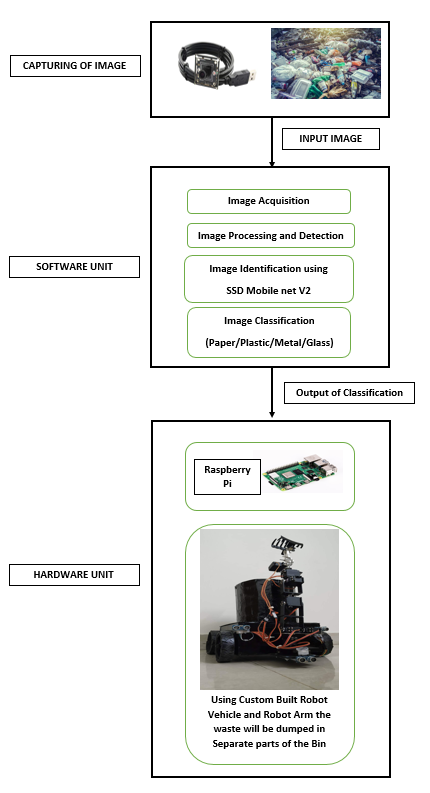
\includegraphics[scale=0.4]{fig.png}}
		\caption{Process of Autonomous Garbage Collection}
		\label{fig}
	\end{figure}
	
	
	\subsection{Usecase/Subsystem}
	
	There are basically two use case for this project. One of them is autonomous and the other is human control.\\
	
	
	\centerline{\textbf {USECASE-1 (AUTONOMOUS)}}
	
	Here the Garbage Collector Robot will be a driverless autonomous vehicle specifically designed to collect waste which require no human intervention. It will automatically detect the waste, move towards it and grab the waste with its robotic arm. Once the waste is collected, it will automatically drop the waste in its specified part(Paper/Plastic/Metal/Glass) of the container.\\
	
	\centerline{\textbf {USECASE-2 (HUMAN CONTROL)}}
	
	Here the Garbage Collector Robot can be controlled manually by a human with the help of an app. The robot can be manually sent front, back, right and left using button controls on the app and can also pickup any waste from the ground using the robotic arm.\\
	
	
	\section{SYSTEM DESIGN / ARCHITECTURE}\label{SCM}
	
	The robot is basically of 4 main parts. At first for the software i.e. the detection part, we used Raspberry Pi which was trained to detect wastes like Paper, Plastic, Metal and Glass. Next, for the movement of the robot we used 4WD robot vehicle that allows the robot to move in any direction it wants to. Thirdly, we attached a Robot Arm to the vehicle which gradually grabs the garbage it detects. Finally, the robot has a rotating bin/basket behind it which collects the garbage grabbed by the robotic arm. So, if paper is collected the basket will rotate to the side of the paper portion of the container and the robot arm will drop the paper in the specific paper part of the basket. As a result, Paper, Plastic, Metal and Glass will be collected separately in different portions of the basket.
	
	\begin{figure}[htbp]
		\centerline{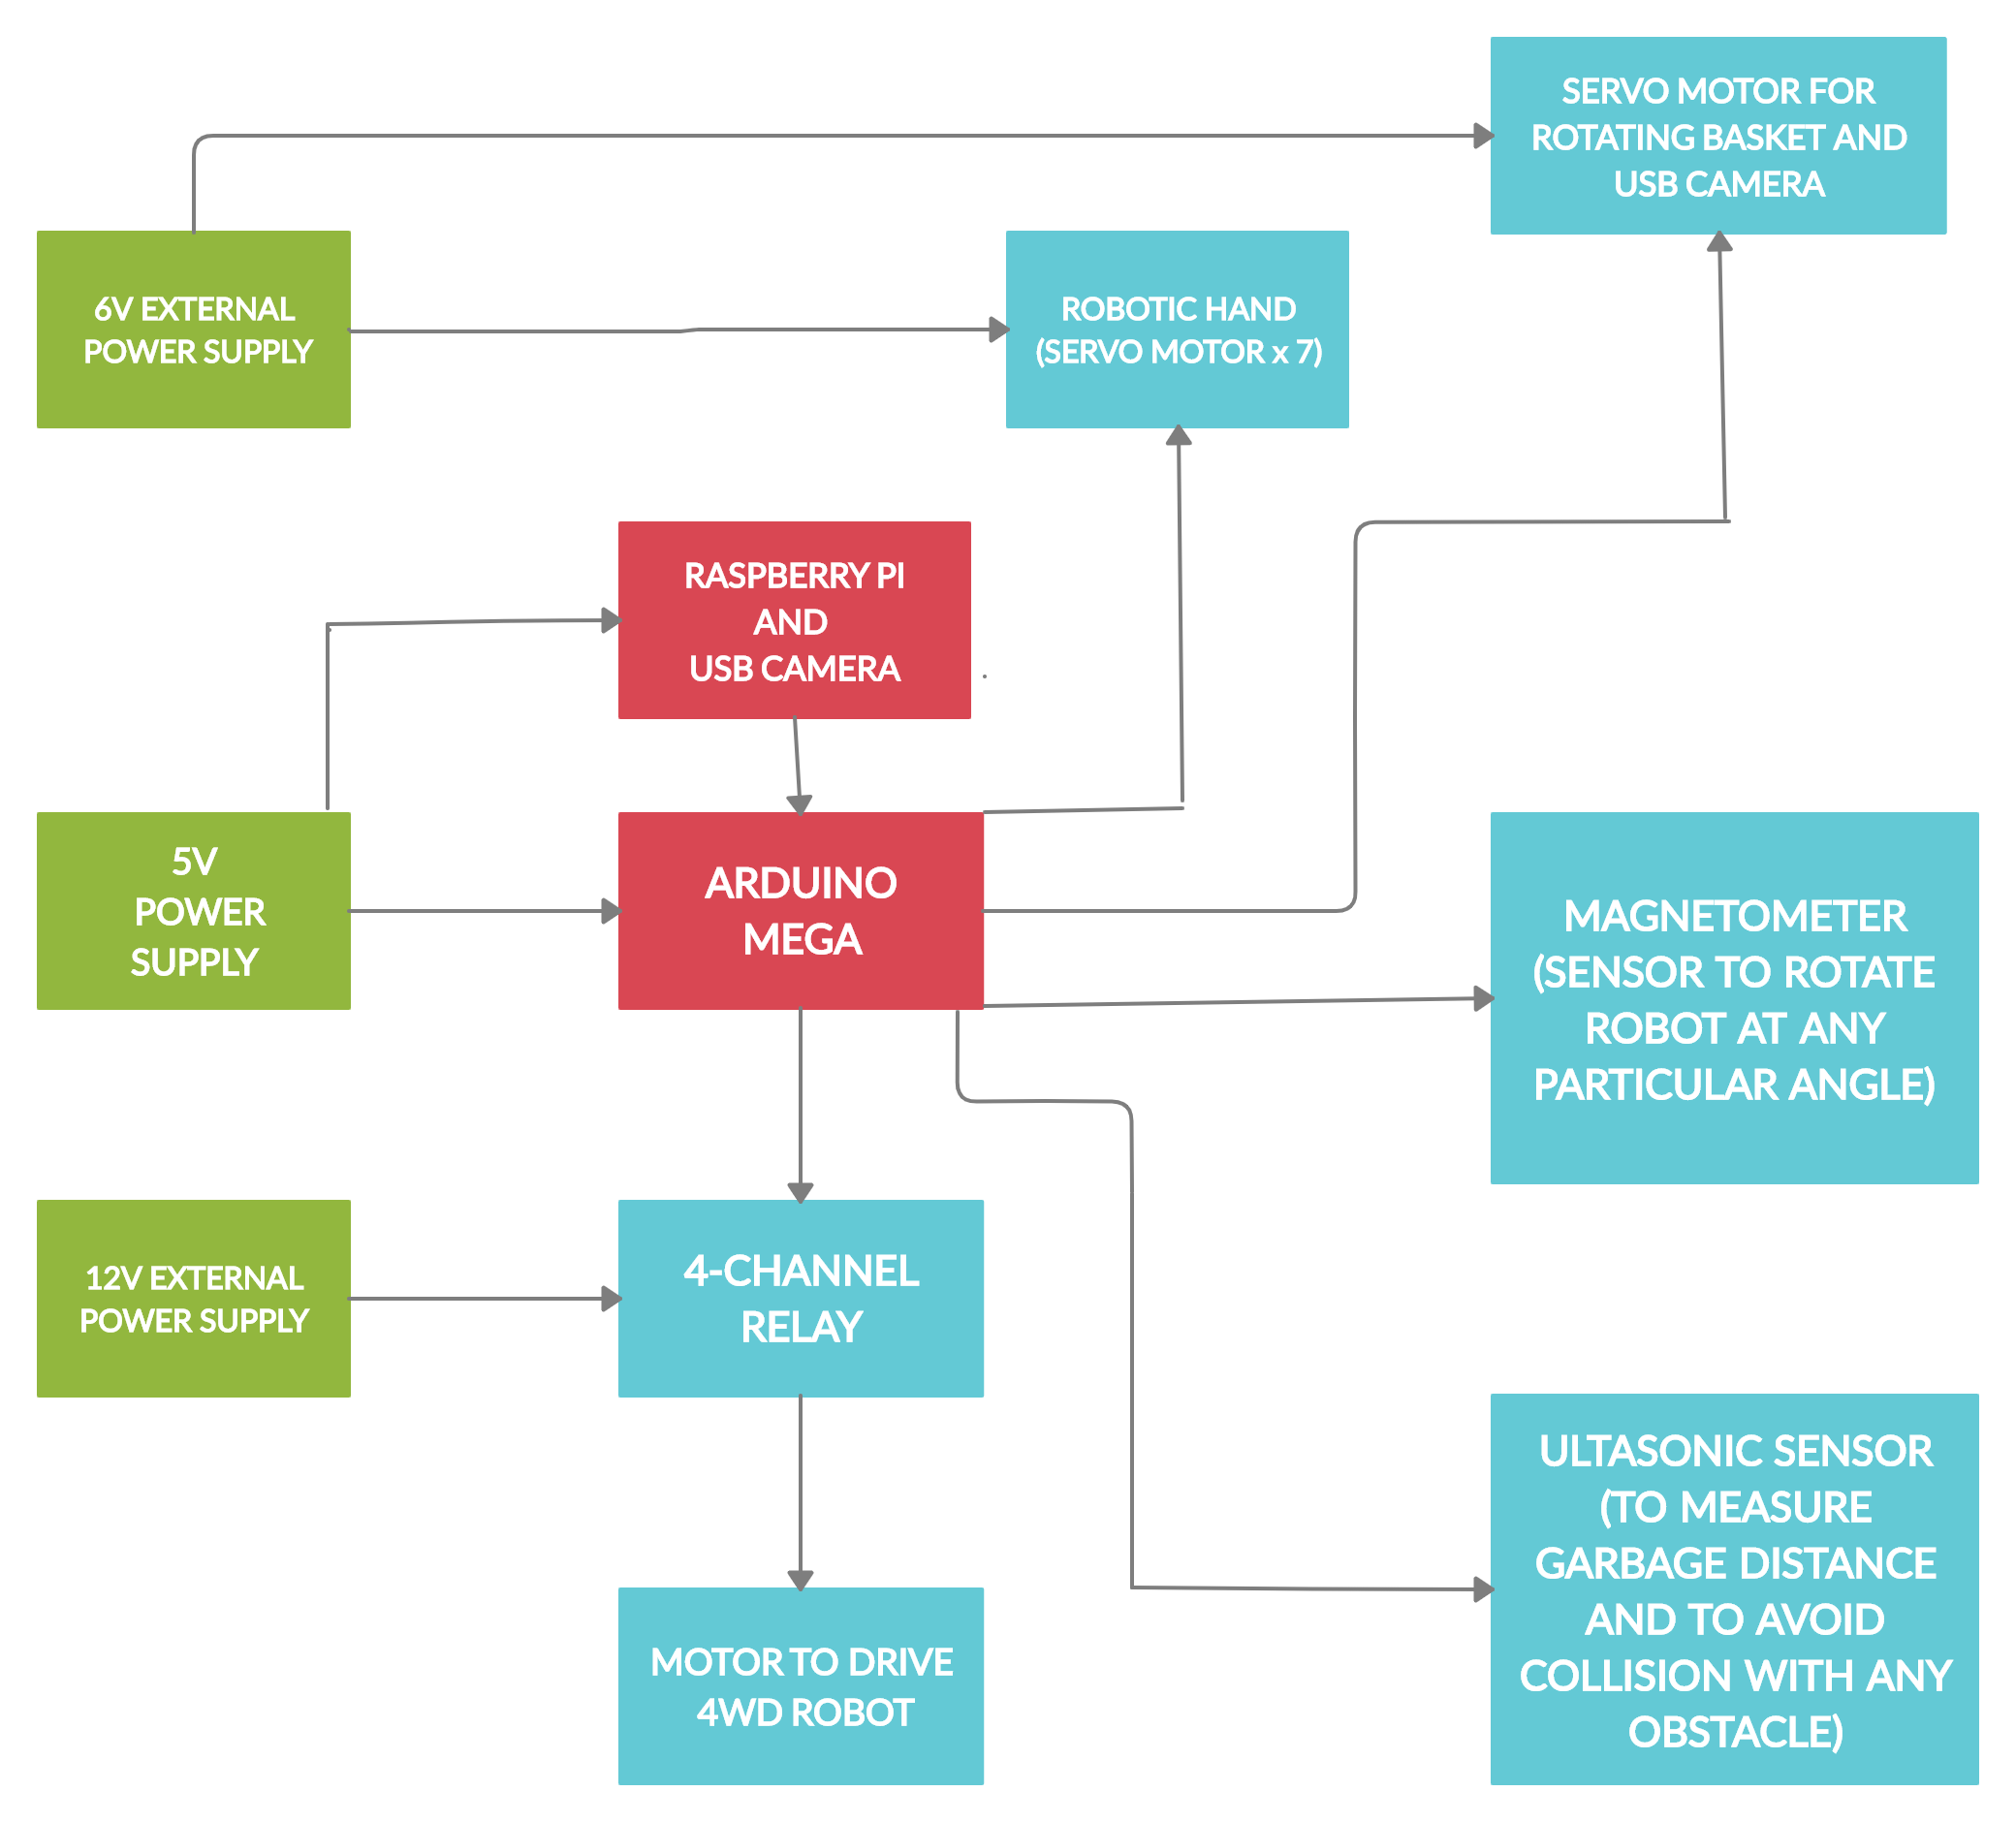
\includegraphics[scale=0.1]{ARCHITECTURE.jpg}}
		\caption{Architecture of Autonomous Garbage Collection Rover}
		\label{fig}
	\end{figure}
	
	\section{USER MANUAL}
	
	Our robot is based on specific conditions like Human Control or Autonomous. A diagram related to its working principle has been generated.
	\begin{figure}[htbp]
		\centerline{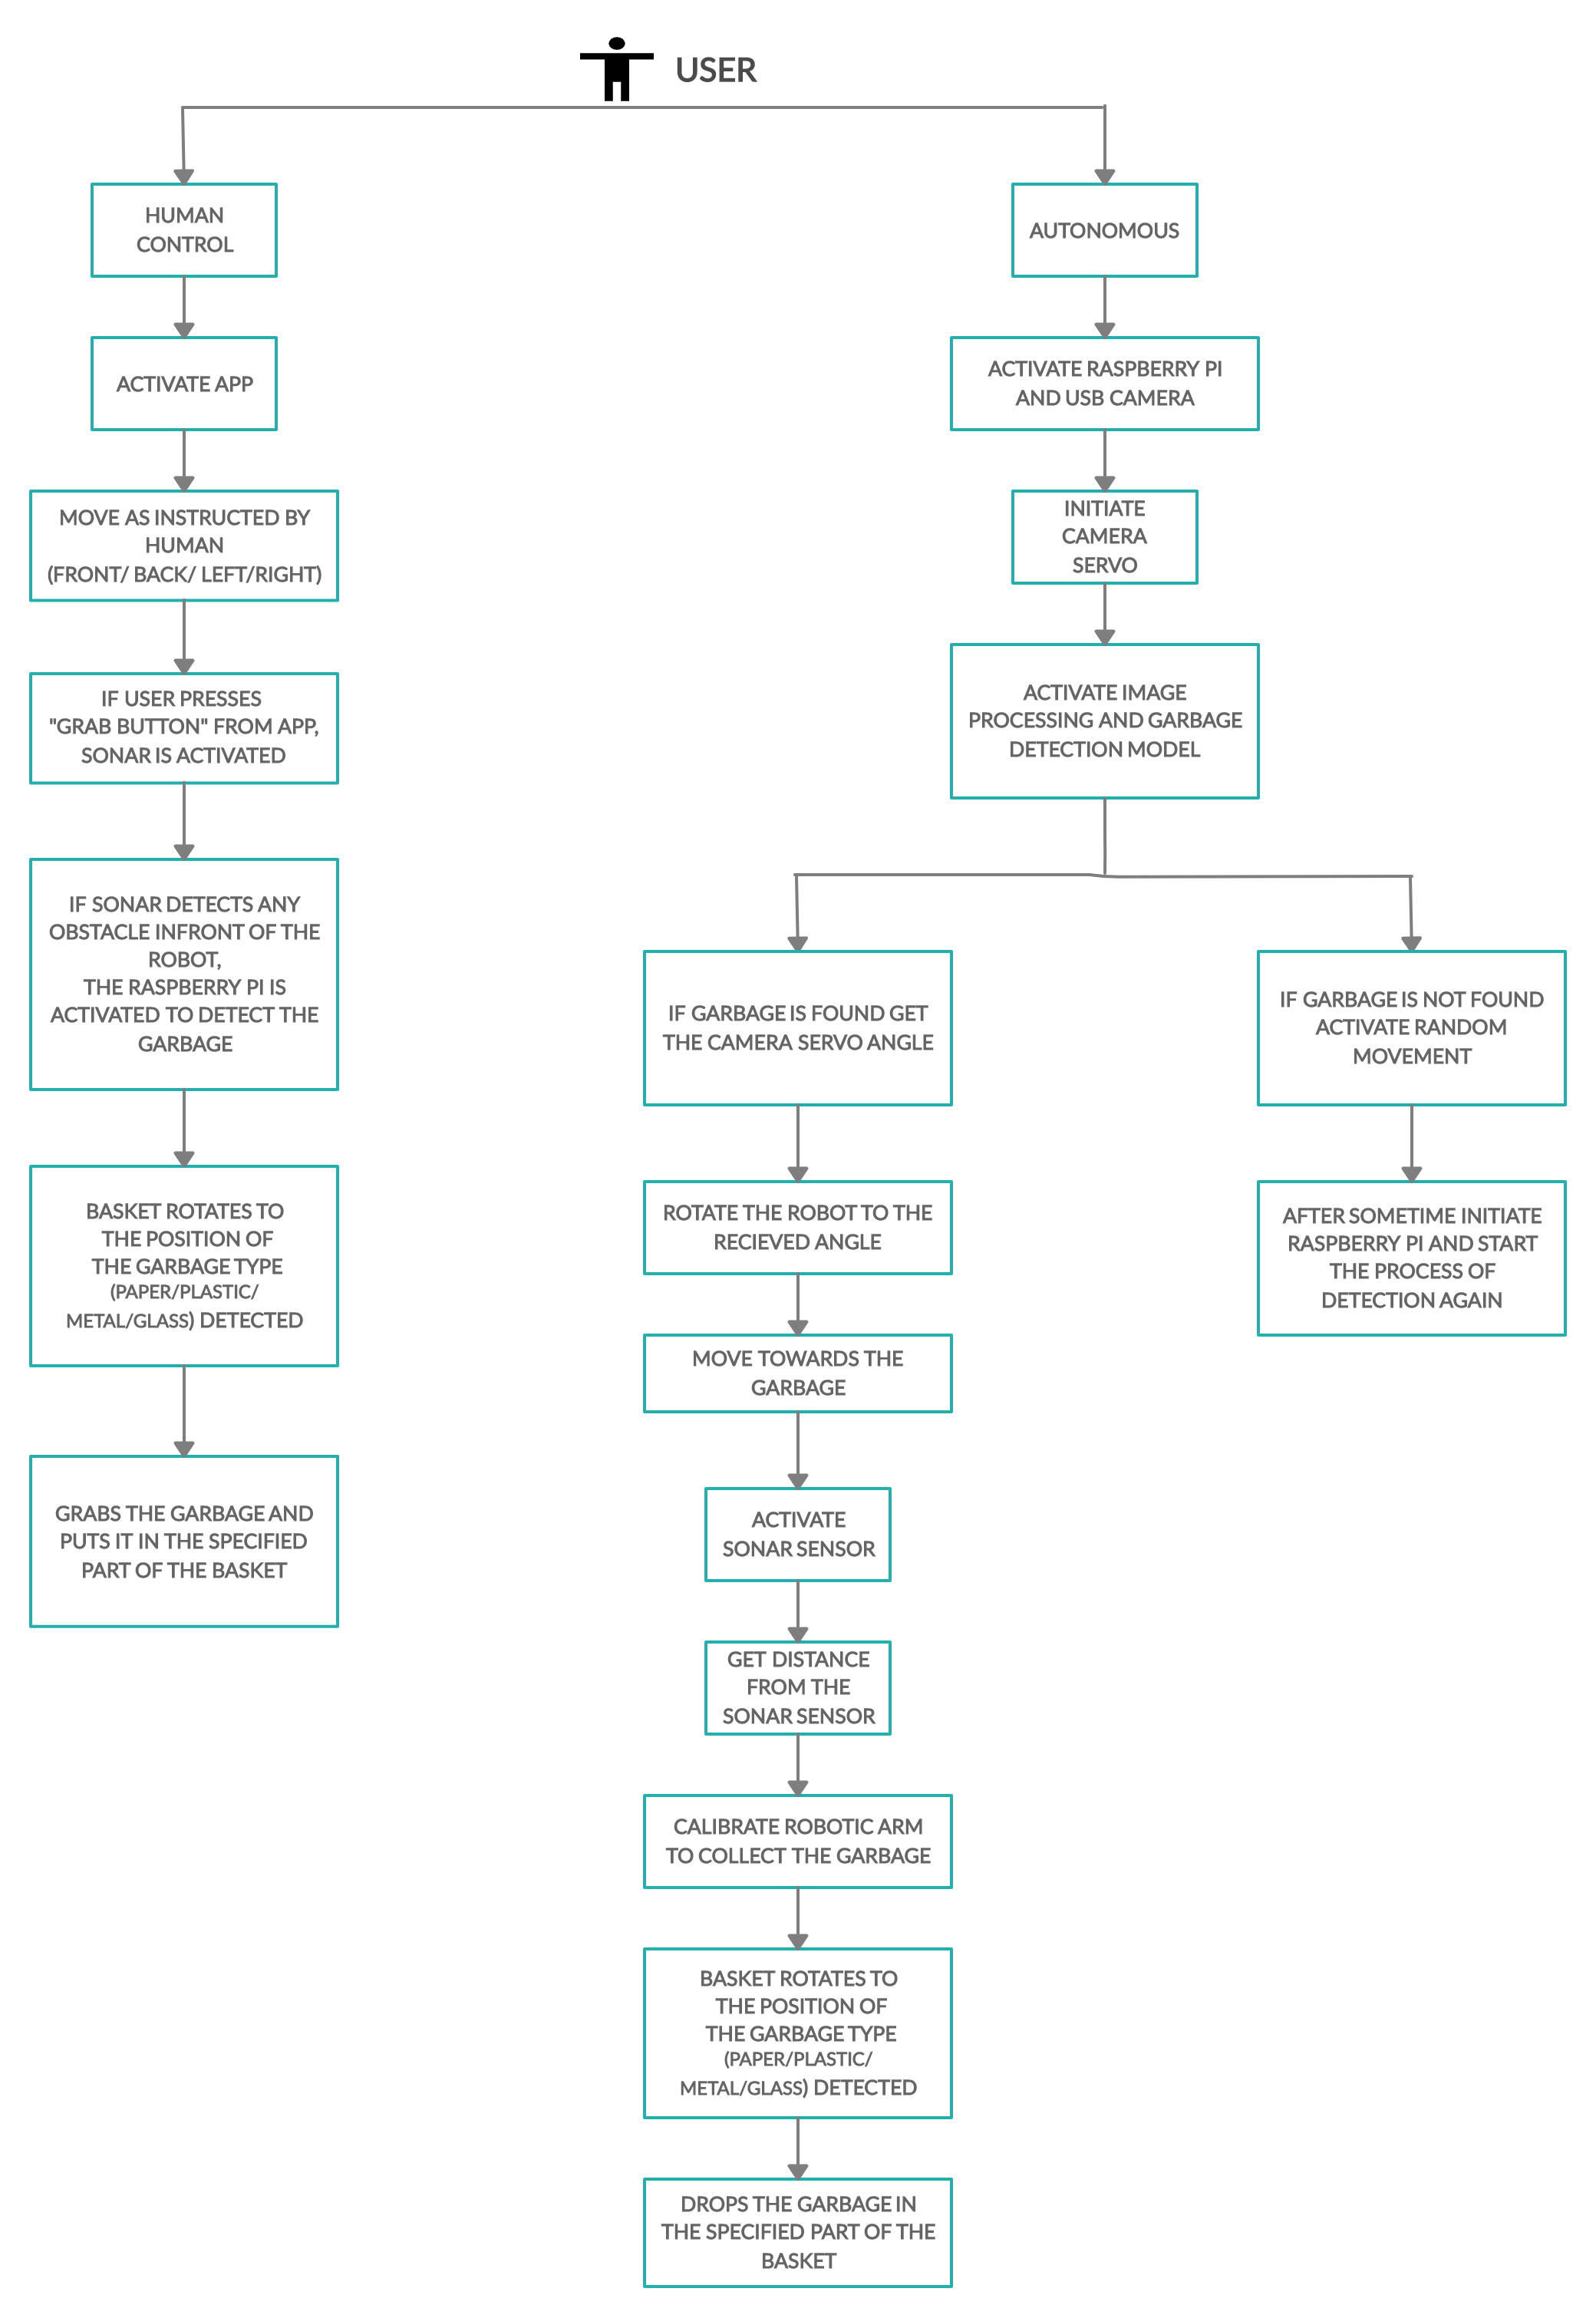
\includegraphics[scale=0.1]{cd.jpg}}
		\caption{User Manual for Autonomous and Human Control Garbage Collector Rover}
		\label{fig}
	\end{figure}
	
	
	\section{SINGLE SHOT MULTIBOX DETECTOR(SSD)— REAL-TIME OBJECT DETECTION IN DEEP LEARNING}
	
	In the field of computer vision, convolution neural networks excel at image classification, which consists of categorising images, given a set of classes and having the network determine the strongest class present in the image. 
	
	\begin{itemize}
		
		\item \textbf{Single Shot: } This means that the tasks of object localization and classification are done in a single forward pass of the network. SSD’s architecture builds on the venerable VGG-16\cite{b6} architecture, but discards the fully connected layers. The reason VGG-16 was used as the base network is because of its strong performance in high quality image classification tasks and its popularity for problems where transfer learning helps in improving results. Instead of the original VGG fully connected layers, a set of auxiliary convolutional layers were added, thus enabling to extract features at multiple scales and progressively decrease the size of the input to each subsequent layer.
		
		\begin{figure}[htbp]
			\centerline{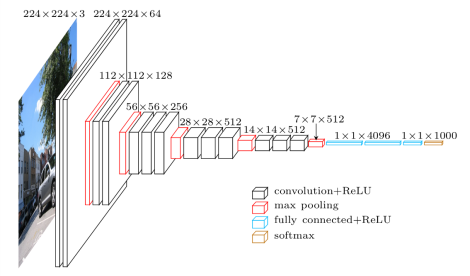
\includegraphics[scale=0.5]{ssd.png}}
			\caption{VGG Architecture}
			\label{fig}
		\end{figure}
		
		
		\item \textbf{Multibox: } MultiBox starts with the priors as predictions and attempt to regress closer to the ground truth bounding boxes. More default boxes results in more accurate detection, although there is an impact on speed. Having MultiBox on multiple layers results in better detection as well, due to the detector running on features at multiple resolutions. 
		
		
	\end{itemize}
	
	\section{ROBOT VEHICLE}
	The robot vehicle is considered to be the main part of the robot. It has customized metal body of Length: 30 cm, Width: 26 cm, Height: 13 cm and Wheel Diameter: 11cm. It is 2 cm above the ground level. All the important devices like Raspberry Pi, Arduino Mega, etc. has been kept inside this vehicle's body. The body contains an extended part in the front to attach the robot arm which will collect the garbage. It has a torque power of 10kg per square cm.
	
	\begin{figure}[htbp]
		\centerline{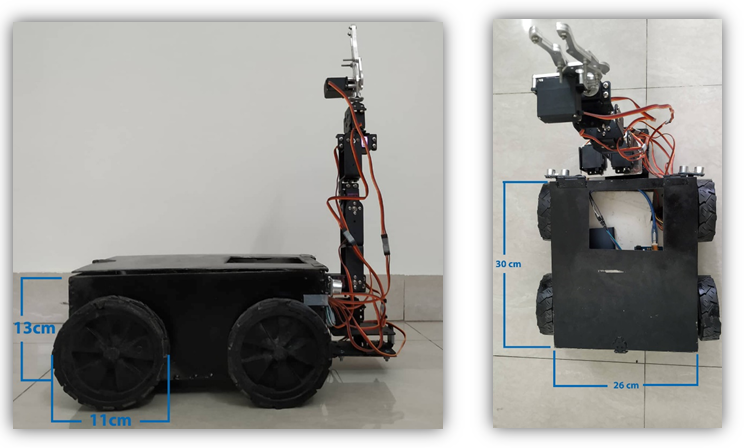
\includegraphics[scale=0.5]{heightlengthwidth.png}}
		\caption{Height, Wheel Diameter, Length and Width of the Robot Vehicle}
		\label{fig}
	\end{figure}
	
	
	\subsection{Motor}
	
	\textbf {Toyota Denso Window Motor:}
	This motor has been used to rotate the wheel of the robot veehicle. It is powerful enough to overcome small or medium sized obstacles. It has a RPM :  80±10rpm (no load) and 55±15rpm (with load)
	\\Max Voltage: 12v
	\\No Load Current: $\le$ 2A
	\\Stall Current: $\le$ 8A  
	\\Rated Torque: 3 N.m $\sim$ 30.6 kg-cm 
	\\Stall Torque: 9.8N.m $\sim$ 100kg-cm.
	
	
	\subsection{Calculations}
	
	Using the right hand rule equation:$\overrightarrow{\rm \tau}=\overrightarrow{\rm \ell}\times\overrightarrow{\rm \digamma}=\digamma\ell\sin\theta\hat{\eta}$
	
	Here, $\rm \tau$ =Torque, moment or moment of force, $\rm \ell$ = Length and $\rm \digamma$= Force\\\\
	When robot is moving forward:
	Direction of F is to the left creating 0-degree angle with the width for Right-sided motors.
	Direction of F is to the left creating 180-degree angle with the width for Left-sided motors.\\
	So, in both cases, length of width is cancelled out as sin(0)=0.
	But, Direction of F is to the left creating 90-degree angle with the length for Right-sided motors.
	Direction of F is to the left creating 90-degree angle with the width for Left-sided motors.
	So, for both cases, torque value should me maximum as sin(90)=1. One Denso motor gives torque of 100 kg-cm. Length of the robot: 30cm\\
	
	So, Maximum weight 1 motor can lift: 100/30 kg =3.3 kg
	\\Maximum weight 4 motor can lift: 3.3kg x 4 = 13.33 kg
	\\Same mechanism for moving backward, right and left.\\
	
	\textbf{Note:} We have tested with 15kg weight above the robot and it worked absolutely fine. So, we can say the motors are much more powerful than it was scripted by the company.
	
	
	\subsection{Power Consumption}
	
	One motor consumes approximately 2$\sim$2.5A depending on its movement. For instance, while moving forward and backward it consumes 2A. On the other hand, while moving right and left it consumes 2.5A. It is because of the drifting of both motor at the opposite directions. While moving right, left sided motors rotate clockwise and right sided motors rotate counter clockwise. To cancel out this opposite direction drifting each motors consumes higher current than moving forward or backward.
	
	So, In total 4 motors consumes: (2$\sim$2.5 x 4)A = 8 $\sim$ 10 A.
	\\We are using 12v 7.5Ah battery. 
	\\So, the uptime of our robot is: 7.5/10 hr = 0.75 hr = 45 mins.
	\\It means, Our robot can be driven up to 45mins straight with full load and working capacity. 
	
	As our battery takes 2A initial current for charging it will take (7.5/2) hr = 3.75 hr = 3hr 45 mins to fully charged. 	
	
	
	\section{ROBOT ARM}
	
	We have run some experiments regarding the grabbing part of the robot arm. The most available servo motor in Bangladesh is MG996R / MG995. Using this servo, it is quite difficult to grab the object from the ground using 6DOF arm. Though we bought 6 DOF arm but we modified the structure of the arm so that it can grab the objects so frequently. So, our custom built robot arm can pick up garbage of a weight limit of 1kg.
	
	\begin{figure}[htbp]
		\centerline{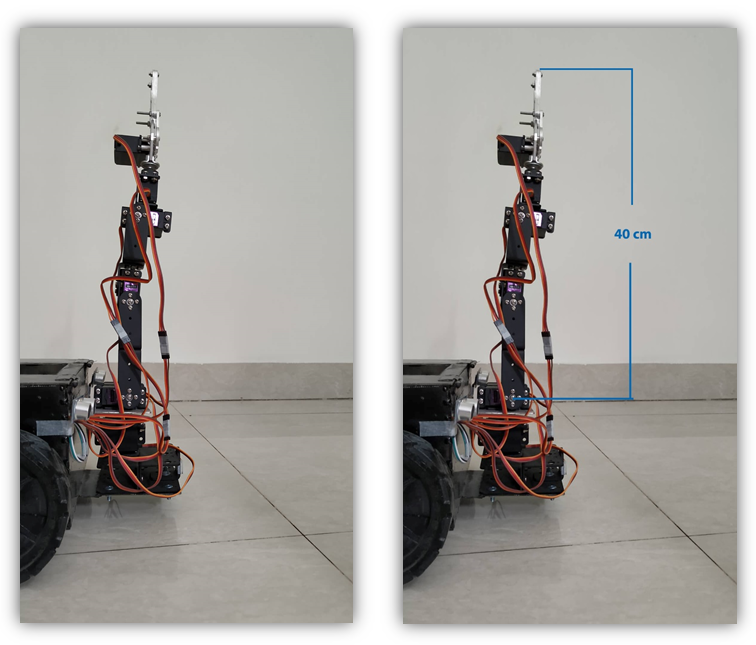
\includegraphics[scale=0.5]{arm.png}}
		\caption{Modified Robot Arm and Robot Arm with required Length}
		\label{fig}
	\end{figure}
	
	
	\subsection{Calculations}
	
	Torque of MG996R: 9.4 kg-cm (at 4.8 v), Torque of MG996R: 11 kg-cm (at 6 v), Operating Voltage: 4.8 v ~ 6.6 v
	\\We are operating at 6 v using 6v 4.5Ah battery. So, we are getting the maximum torque of 11kg-cm.
	
	
	\subsection{Torque Equation}
	
	Using the right hand rule equation:$\overrightarrow{\rm \tau}=\overrightarrow{\rm \ell}\times\overrightarrow{\rm \digamma}=\digamma\ell\sin\theta\hat{\eta}$
	
	Here, $\rm \tau$ =Torque, moment or moment of force, $\rm \ell$ = Length and $\rm \digamma$= Force\\
	The length from Shoulder (Servo2) to the gripper top is: $\sim$40 cm. Maximum weight that 1 MG996R servo can lift: 11 kg-cm / 40 cm = 275 gm
	\\So, total weight shoulder servos can lift:275 $\times$ 2 gm = 550 gm. Equipment’s total weight above Servo2 : \\Weight of Claw + Weight of U Bracket $\times$ 3  + MG996R servo $\times$ 4 + Multifunctional Bracket $\times$ 3 + L-type Bracket $\times$1
	
	= (56 + 22 $\times$ 3 + 55 $\times$ 4 + 16 $\times$ 3 + 6) gm 
	
	= 396 gm, which is greater than 275 gm but less than 550gm
	
	So, Shoulder servos can lift total weight of garbage = (550 – 396) gm = 104 gm which is enough for our project. 
	
	\subsection{Modifications Necessary}
	
	If we used 1 servo in the shoulder of the 6 DOF then the height from shoulder to the gripper top would be still approximately 40 cm. 
	Then it can lift maximum weight of = 11 kg-cm / 40 cm =0.275 kg  $\sim$275 gm.\\
	But component’s total weight above Shoulder would be 
	= (56 + 22 $\times$ 3 + 55 $\times$ 4 + 16 $\times$ 3 + 6) gm 
	= 396 gm which is greater than 275 gm.
	So, it will not work properly.\\ 
	
	\textbf{Note:} We ran some tests earlier on 6DOF and we saw that Shoulder servo falls down with the excessive weight as it’s torque is not compatible with that much weight. 
	So, we modified and used two servos together in the shoulder with the help of a customized metallic plate. After modification, our robot arm can grab the garbage and lift it properly. As our robotic hand is compatible with XYZ (3D) rotation so it is enough for our project. 
	
	
	\subsection{Power Consumption}
	
	We have used 7 servos for robotic hand, 1 servo to rotate the basket, 1 for rotating camera. So in total 9 servos are used. 
	Each servo has a stall current of 1.4 A. 
	So total Stall current: (9 $\times$ 1.4) A = 12.6 A
	We are using 6v 4.5Ah to power up the robot arm servos along with basket servo and camera servo.
	So the uptime of robotic hand and basket and camera rotation function is: (4.5/12.6) hr = 0.38 hour $\sim$ 22 mins.
	This is the uptime with full load functionalities. All the servos will not work at full load capacity because of their position. Neither all the servos are at the maximum distance from the gripper of the robotic hand nor they lift the maximum weight while picking garbage. So power(current) consumption is not equal for all the servos. We noticed that the actual uptime is almost triple of this time which is more than enough for our project. 
	The idle current draw for each servo: 10mA which is so low and we can ignore it.  
	
	
	\section{FEATURES}
	\begin{itemize}
		
		\item \textbf{Obstacle Avoidance:} There are 3 sonar sensors in the front and 1 at the back of the robot vehicle to avoid obstacles in the pathway of the robot. The sonars in the front can rotate from 0 to 90 degrees with the help of the servo which helps the sonar sensors to increase the range of coverage on the left and right side of the robot. IR sensors are also used to put firm in the obstacle avoidance functionality. There is a IR sensor on the robotic arm at height 35cm just below the claw. This sonar helps to avoid any obstacle present in the range of the height of the robot arm.
		
		
		\item \textbf{Living Beings Avoidance: } There is a PIR motion sensor in the front of the robot. A passive infrared sensor (PIR) is an electronic sensor that measures infrared light radiating from objects in its field of view. It helps to detect any kind of movement in front of the robot and avoid it. A Thermal sensor (OMRON MEMS) is combined with PIR sensor in order to detect living being more precisely.
		\\
		\textbf{Future Improvement: “Detect living being from webcam through image processing.”}
		
		
		\item \textbf{Movement Accuracy:} The robot is based on image processing. So it will get a direction from the camera servo. Initially the camera servo starts rotating and if it detects any garbage nearby it will send the camera servo angle to the Arduino. Depending on the motor rpm robot will get an initial rotation time to rotate in that direction given by camera servo. While rotating the MPU6050 sensor (gyroscope, accelerometer) will confirm the rotation. As the robot moves forward both IR and Sonar sensor will confirm the remaining distance of the garbage from the robot. 
		
		
		\item \textbf{Security:} A GPS is attached to the rover so that we can identify its location through google map. It is very important as any autonomous robot can be misused and stolen if we don’t use GPS system. For example: If anyone picks up the robot and takes it out from it designated coordinates, a notification will be sent to the control. Besides, we can also detect whether the robot is working properly or not by seeing its location. For example: During autonomous mode if the robot is stuck in a specific location for more than 2 minutes, a notification will be automatically sent to the control room.
		
		
		\item \textbf{Live Feedback:} If there will be any sort of misbehaviour from the robot the system will identify it and sends a message to the control room with the help of Arduino and SIM900A module. A sim card will be inside the module and it will send the error message to the control room. 
		
		
		\item \textbf{High Power Motors:} High Power Motors which helps to move over small or medium sized objects.
		Maximum weight 4 motor can lift: 3.3kg x 4 = 13.33 kg. Since out robot is 6kg, it can easily move around its environment without any difficulties.
		
		
		\item \textbf{Future Implementation:}
		
		\begin{itemize}
			
			\item 
			Using Reinforcement Machine Learning Algorithm the robot will be taught the surrounding environment and will make its own decision whether to move next after grabbing one garbage. Obviously there will be an increase number of sensors to support this mechanism.
			
			
			\item
			Add solar chargers to the robot so that it can automatically charge itself when it runs out of power.
			
			\item
			Improve dataset by adding more images to it. This will increase the detection and accuracy level to a great extent. 
			
		\end{itemize}
		
	\end{itemize}
	
	\section*{CONCLUSION}
	
	This system isolates waste automatically utilizing sensors, motors and detection software.The proposed system concentrates on identification, classification and segregation of waste. As the system works independently, there is no need of human mediation to control or to do any assignment. Utilizing Raspberry Pi and USB camera, the characterization result of images taken will automatically categorize the garbage as Plastic, Paper, Glass and Metal and send signals to the robot to collect the garbage. Once our modified robot gets the signal it will move towards the garbage and collect it using the modified robot arm. Finally the garbage will be dumped in separate portions of a basket based on the type of garbage collected. Our robot is different from other garbage collector robots as it can run in any unknown location. Sonar sensors allow it to avoid obstacles. Moreover, we used SSD Mobile Lite for detection of garbage which has lower processing power but great detection level. As a result, it will not heat up the processor of Raspberry Pi allowing it to run smoothly.
	
	
	
	\begin{thebibliography}{00}
		\bibitem{b1} Nurlansa, Osiany, Dewi Anisa Istiqomah, and Mahendra Astu Sanggha Pawitra. "AGATOR (automatic garbage collector) as automatic garbage collector robot model." International Journal of Future Computer and Communication 3.5 (2014): 367.
		
		\bibitem{b2}Wattanasophon, S., and Sarinee Ouitrakul. "Garbage collection robot on the beach using wireless communications." Int. Proc. Chem. Biol. Environ. Eng 66 (2014): 92-96.
		
		\bibitem{b3}Rama Prabha, D., Mahindru, S., Srivastava, A.,  Nilalohita, P. AUTONOMOUS GARBAGE COLLECTOR–ROBODUMPSTER.
		
		\bibitem{b4}Ferri, G., Manzi, A., Salvini, P., Mazzolai, B., Laschi, C.,  Dario, P. (2011, May). DustCart, an autonomous robot for door-to-door garbage collection: From DustBot project to the experimentation in the small town of Peccioli. In 2011 IEEE International Conference on Robotics and Automation (pp. 655-660). IEEE.
		
		\bibitem{b5} Available: https://www.kaggle.com/asdasdasasdas/garbage-classification
		
		\bibitem{b6}Liu, W., Anguelov, D., Erhan, D., Szegedy, C., Reed, S., Fu, C. Y.,  Berg, A. C. (2016, October). Ssd: Single shot multibox detector. In European conference on computer vision (pp. 21-37). Springer, Cham.
		
		\bibitem{b7}Jha, A., Singh, A., Kerketta, R., Prasad, D., Neelam, K.,  Nath, V. (2019). Development of Autonomous Garbage Collector Robot. In Proceedings of the Third International Conference on Microelectronics, Computing and Communication Systems (pp. 567-576). Springer, Singapore.
		
		\bibitem{b8}Simoes, A. S., Carrion, R., Martins, A. C., Costa, R. B., Schvarcz, A. F., Buzo, V. R., ...  Ferrari, B. A. (2006, October). Autonomous mobile robots designing for the medical trash collector task. In 2006 IEEE 3rd Latin American Robotics Symposium (pp. 234-239). IEEE.
		
		\bibitem{b9}Parashar, S.,  Tomar, P. Waste Management by a Robot-A Smart and Autonomous.
		
		\bibitem{b10}Hossain, S., Debnath, B., Anika, A., Junaed-Al-Hossain, M., Biswas, S.,  Shahnaz, C. (2019, October). Autonomous Trash Collector Based on Object Detection Using Deep Neural Network. In TENCON 2019-2019 IEEE Region 10 Conference (TENCON) (pp. 1406-1410). IEEE.
		
	\end{thebibliography}
	\vspace{12pt}
	
	
\end{document}
